\section{Análisis de componentes principales}
\label{resultados:pca}

\subsection{Conjunto de datos completo}

\paragraph{}
Para este caso, al ejecutar el \textit{PCA} con el conjunto de datos completo, este nos muestra tal y como podemos ver en la figura \ref{pcaOneResult}, que \textbf{con solo 3 atributos}, el modelo es \textbf{capaz de explicar (predecir) el 95\% de las observaciones}.

\begin{figure}[!htb]
  \centering
    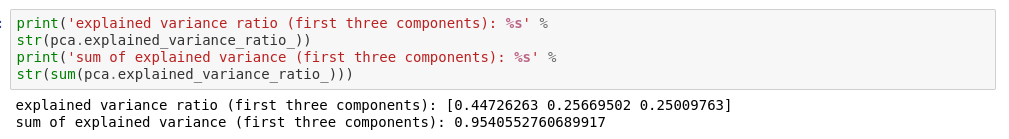
\includegraphics[width=0.9\textwidth]{images/resultados_procesado_de_datos_pca1_result.png}
    \caption{Resultado del \textit{PCA}.}
  \label{pcaOneResult}
\end{figure}

\paragraph{}
Dado que el \textit{PCA} solo nos muestra 3 atributos como relevantes, podemos representar los resultados de las observaciones a un gráfico que mostramos en la figura \ref{pcaOneGraphic} dibujando los 3 componentes principales como si fueran 3 dimensiones, y pintamos los valores a predecir sobre estos (aplicando el color rojo a las observaciones que no consideran útiles, y azul a los que si se consideran útiles), podemos observar que la gran mayoría de los rojo se encuentran en el plano del componente principal 1 y 2, mientras que el azul esta más repartidos en los dos planos.

\begin{figure}[!htb]
  \centering
    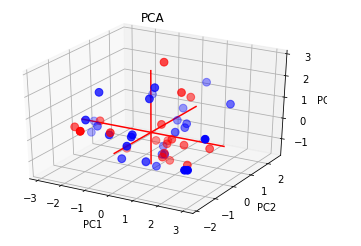
\includegraphics[width=0.4\textwidth]{images/resultados_procesado_de_datos_pca1_graphic.png}
    \caption{Proyección delos resultados del \textit{PCA} en una gráfica.}
  \label{pcaOneGraphic}
\end{figure}

\paragraph{}
Si le pedimos al modelo que nos indique cuales son los 3 componentes que ha detectado que son los principales, este nos muestra los resultados que se pueden ver en la figura \ref{pcaOneAtributos}. Para saber cuales son los componentes, tendremos que quedarnos para cada componente principal, el valor del atributo que más se acerque a 1.

\begin{figure}[!htb]
  \centering
    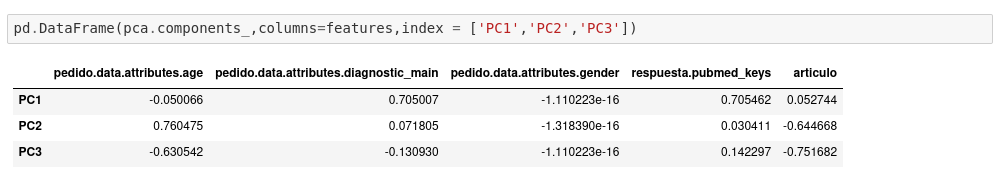
\includegraphics[width=0.9\textwidth]{images/resultados_procesado_de_datos_pca1_atributos.png}
    \caption{Proyección de los resultados del \textit{PCA} sobre los atributos del conjunto de datos.}
  \label{pcaOneAtributos}
\end{figure}

\paragraph{}
Para este caso, el \textit{PCA} nos muestra que \textbf{los 3 componentes principales son, el atributo \textit{pubmed\_keys}, el atributo \textit{age} y el atributo \textit{diagnostic\_main}}.

\subsection{Conjunto de datos solo con atributo utilidad definido}
\label{result:pca_case2}
\paragraph{}
En este caso, el \textit{PCA} nos muestra tal y como podemos ver en la figura \ref{pcaTwoResult}, que \textbf{necesitamos 5 atributos} para que el modelo sea \textbf{capaz de explicar (predecir) el 97\% de las observaciones}.

\begin{figure}[!htb]
  \centering
    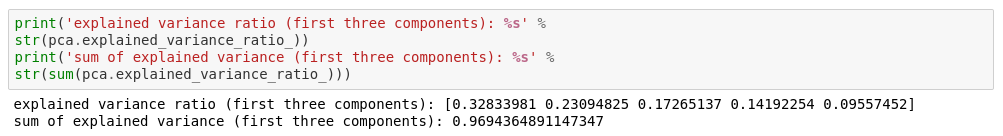
\includegraphics[width=0.9\textwidth]{images/resultados_procesado_de_datos_pca2_result.png}
    \caption{Resultado del \textit{PCA} de la segunda ejecución.}
  \label{pcaTwoResult}
\end{figure}

\paragraph{}
Para este caso, el \textit{PCA} nos muestra tal y como podemos ver en la figura \ref{pcaTwoAtributos}, que los \textbf{5 componentes principales} son, \textbf{el atributo \textit{diagnostic\_main}, el atributo \textit{Year}, el atributo \textit{pubmed\_keys}, el atributo \textit{age} y el atributo \textit{artículo}}.

\paragraph{}
La diferencia del número de atributos necesarios que nos muestra el \textit{PCA} respecto al conjunto anterior seguramente este debido a que el conjunto completo contiene un gran volumen de observaciones con el atributo '\textit{utilidad}' sin definir, lo que hace que prácticamente cualquier valor que tengan los atributos se acaben asociando a un resultado sin definir, como pasa en el conjunto de datos original. Al no tener en cuenta las observaciones con el atributo '\textit{utilidad}' sin definir, el \textit{PCA} ya nos indica que necesita analizar más atributos para acabar explicando el valor final.

\begin{figure}[!htb]
  \centering
    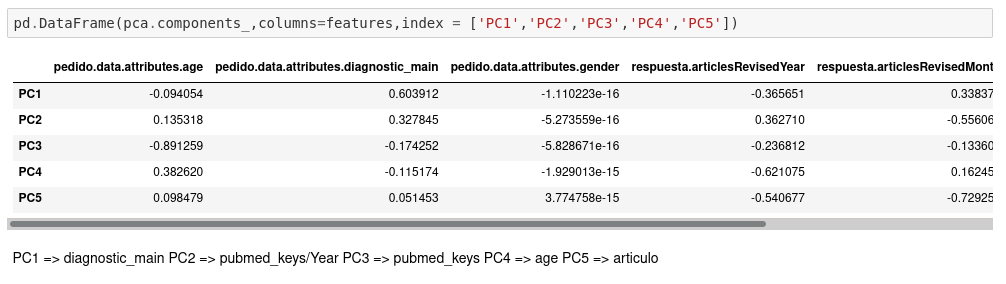
\includegraphics[width=0.9\textwidth]{images/resultados_procesado_de_datos_pca2_atributos.png}
    \caption{Proyección de los resultados del \textit{PCA} sobre los atributos del conjunto de datos para la segunda ejecución.}
  \label{pcaTwoAtributos}
\end{figure}

\subsection{Conjunto de datos solo con atributo utilidad definido, añadiendo el mes y año del artículo, eliminando los atributos \textit{gender} y artículo y expandiendo el atributo \textit{respuesta.pubmed\_keys}}
\label{result:pca_case3}
\paragraph{}
En este caso, el \textit{PCA} nos muestra tal y como podemos ver en la figura \ref{pcaThreeResult}, que \textbf{necesitamos 4 atributos} para que el modelo sea \textbf{capaz de explicar (predecir) el 90\% de las observaciones}.

\begin{figure}[!htb]
  \centering
    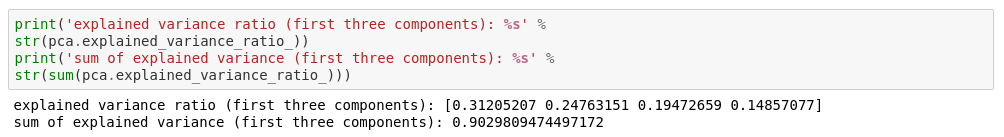
\includegraphics[width=0.9\textwidth]{images/resultados_procesado_de_datos_pca3_result.png}
    \caption{Resultado del \textit{PCA} de la tercera ejecución.}
  \label{pcaThreeResult}
\end{figure}

\paragraph{}
Para este caso, el \textit{PCA} nos muestra como podemos ver en la figura \ref{pcaThreeAtributos} , que los \textbf{4 componentes principales} son, \textbf{el atributo \textit{diagnostic\_main}, el atributo \textit{Month}, el atributo \textit{pubmed\_keys} y el atributo \textit{age}}.

\begin{figure}[!htb]
  \centering
    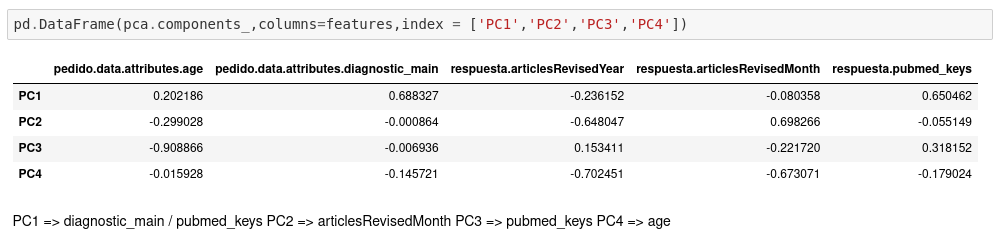
\includegraphics[width=0.9\textwidth]{images/resultados_procesado_de_datos_pca3_atributos.png}
    \caption{Proyección de los resultados del \textit{PCA} sobre los atributos del conjunto de datos para la tercera ejecución.}
  \label{pcaThreeAtributos}
\end{figure}
